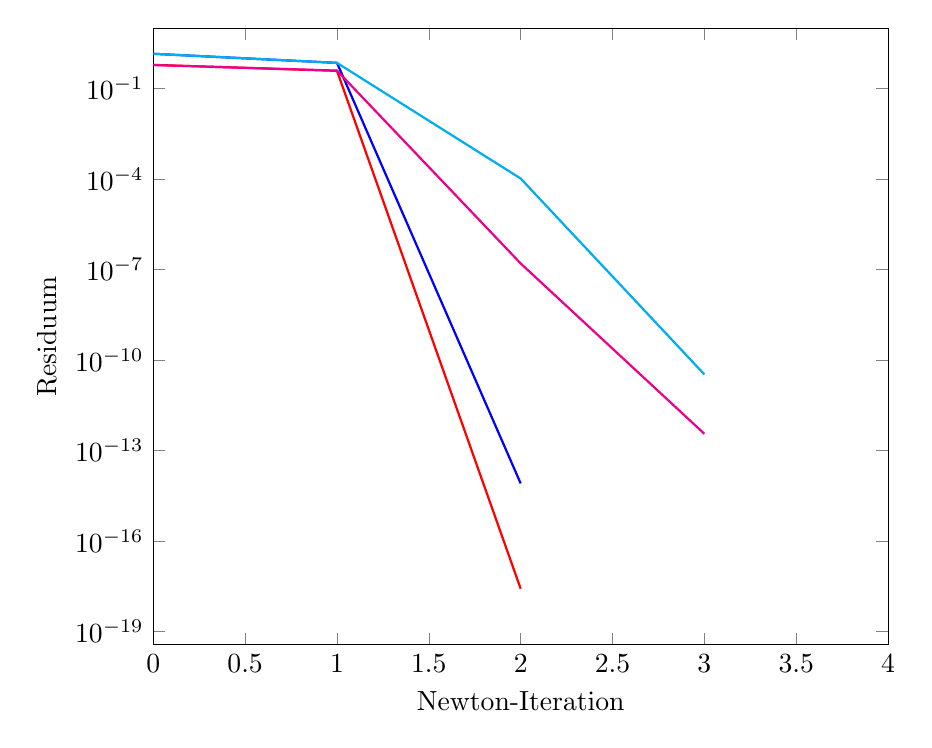
\begin{tikzpicture}[every plot/.append style={thick}] 
\begin{axis}[ 
label style={font=\normalsize}, 
xlabel={Newton-Iteration}, 
ylabel={Residuum}, 
xmin=0, xmax=4, 
ymode=log, 
ymin=0, ymax=10, 
width=0.9\textwidth, 
grid style=dashed, 
] 
\addplot[ 
color=blue, 
] 
coordinates { 
(0, 1.42e+00)(1, 7.10e-01)(2, 8.09e-15)}; 
\addplot[ 
color=red, 
] 
coordinates { 
(0, 6.09e-01)(1, 3.86e-01)(2, 2.61e-18)}; 
\addplot[ 
color=cyan, 
] 
coordinates { 
(0, 1.42e+00)(1, 7.10e-01)(2, 1.04e-04)(3, 3.34e-11)}; 
\addplot[ 
color=magenta, 
] 
coordinates { 
(0, 6.03e-01)(1, 3.94e-01)(2, 1.59e-07)(3, 3.58e-13)}; 
\end{axis} 
\end{tikzpicture} 
